\documentclass[11pt,a4paper]{article}

\usepackage[margin=2.3cm]{geometry}
\usepackage{amsmath,amssymb}
\usepackage{graphicx}
\usepackage{booktabs}
\usepackage{enumitem}
\usepackage[hidelinks]{hyperref}
\usepackage{caption}

\emergencystretch=1.5em
\captionsetup{font=small,labelfont=bf,width=.95\textwidth}
\setlength{\parskip}{4pt plus 1pt}
\setlength{\parindent}{0pt}

\newcommand{\code}[1]{\texttt{#1}}
\newcommand{\TopK}{\operatorname{TopK}}
\newcommand{\sg}{\operatorname{sg}}

\title{Gumbel Top-$(K{+}J)$ versus hard Top-$K$,\\
with the code carried between blocks\\[2pt]
\large Research note}
\author{}
\date{2026-11-13.}

\begin{document}
\maketitle
\vspace{-2em}

% ============================================================
\section{Purpose and summary of conclusions}
% ============================================================

Three questions: does a Gumbel Top-$(K{+}J)$ bottleneck, trained with a policy
gradient, beat hard Top-$K$; which candidate pool $J$ is best; and how should the
temperature $\tau$ and the policy coefficient $\lambda$ be set. All runs use
abs-TopK selection (Section~\ref{sec:setup}); runs with separately computed
selection scores did not train and were paused
(\code{docs/separate-score-failure.pdf}).

\begin{itemize}[leftmargin=1.2em,itemsep=3pt]
\item \textbf{Gumbel Top-$(K{+}J)$ does not beat hard Top-$K$.} All 27 tuned
  20000-step cells (9 $(K,J)$ pairs $\times$ 3 sampling variants) end within
  $-0.001$ to $+0.018$ nats of hard Top-$K$ at the same $K$, and $0.05$ to $0.26$
  above hard Top-$(K{+}J)$. On the hard ladder every cell sits at the Top-$K$
  end of the interval between hard Top-$K$ and Top-$2K$ (one doubling of $K$
  is worth $0.03$--$0.09$ nats).
\item \textbf{$J$ does not matter.} At each $K$ and variant the final CE over
  $J$ spans at most $0.011$ nats. Only with all 8 bottlenecks sampling is one
  pool consistently best: the narrowest, $J = K$, by up to $0.01$.
\item \textbf{The policy term only hurts.} At step 2500 the loss rises
  monotonically with $\lambda$ for every $\tau$ (mean over cells). In the first
  grid, $\lambda = 10^{-2}$ and $10^{-1}$ collapsed training to the unigram level
  (CE $\approx 6$), and $\lambda = 1$ did so in a 30-step smoke test;
  $\lambda = 10^{-3}$ collapsed by step 1000. The selected
  setting is $\lambda = 0$ in all 27 cells: Gumbel noise on the support, no
  policy gradient.
\item \textbf{Smallest temperature.} $\tau = 0.2$ is selected in 23 of 27
  cells, $\tau = 0.5$ in the other 4; $\tau = 1.2$ costs $0.04$--$0.12$ nats at
  step 2500 (mean over cells).
\item \textbf{Sampling at 3 of 8 bottlenecks} roughly halves the cost of a
  given $\lambda$ (mean margin $+0.41$ instead of $+0.80$ at $\tau = 0.5$,
  $\lambda = 10^{-4}$) and ties sampling at all 8 at $\lambda = 0$. Drawing the 3
  bottlenecks once per forward or separately per token gives the same results
  within $0.01$ nats.
\end{itemize}

% ============================================================
\section{Setup}\label{sec:setup}
% ============================================================

\textbf{Model.} 8 blocks of width 768 on TinyStories, an activation bottleneck
after every block (\code{residual\_out}, $N = 1536$ coordinates), code carried
between blocks (\code{code\_residual: true}), no output norm, magnitude--direction
decoupling, batch $96 \times 512$, seed 1337. Unlike the K+J notes, the learning
rate is \emph{constant} at $6\cdot10^{-4}$ after a 500-step warmup
(\code{configs/gumbel\_cr/base.yaml}). The bottleneck at block $l$ keeps the
support $S_l$ of $K$ coordinates of the code $a_l$ (abs-TopK: the $K$ largest
$|a_{l,i}|$); the hard Top-$K$ baselines train with that deterministic support,
$K \in \{16, 32, 64, 128, 256\}$.

\textbf{Gumbel Top-$(K{+}J)$.} In training each bottleneck draws its support
from the candidate pool $C = \operatorname{TopIndices}_{K+J}(|a|)$,
\begin{equation}
  S = \TopK_K\!\big(|a|_C/\tau + G_C\big), \qquad G_i \sim \mathrm{Gumbel}(0,1),
\end{equation}
independently per sequence, position and bottleneck, and the trainer adds the
policy term
\begin{equation}
  \lambda \textstyle\sum_b w_b\, \sg(\ell_b - \beta_b)\, P_b
\end{equation}
to the CE: $\ell_b$ is the CE of sequence $b$, $\beta_b$ the mean CE of the other
sequences of its micro-batch (leave-one-out baseline), $P_b$ the sequence's
summed ordered Plackett--Luce log-probability of its draws, and $w_b$ its weight
in the CE. Validation uses the deterministic Top-$K$. The coordinates kept carry
their values unscaled.

\textbf{Variants.} All 8 bottlenecks sample (\code{gcr\_gum\_*}); or 3 of the 8,
drawn uniformly once per forward (\code{gcr\_gum3f\_*}) or once per position
(\code{gcr\_gum3t\_*}), the other 5 using their deterministic Top-$K$.

\textbf{Grid and search.} $(K, K{+}J) \in \{16\}\times\{32,64,128,256\} \cup
\{32\}\times\{64,128,256\} \cup \{64\}\times\{128,256\}$. At each of the 9
cells and each variant, $\tau \in \{0.2, 0.5, 1.2\}$ (at initialization these
put about 9\,\%, 27\,\% and 63\,\% of the drawn support outside Top-$K$ at
$K = 32$, pool $N$) and $\lambda \in \{0, 10^{-5}, 3\cdot10^{-5}, 10^{-4}\}$.
Search runs stop at step 2500; under the constant learning rate they are the
first 2500 steps of the full run, and the setting with the lowest validation CE
at step 2500 is resumed from its own checkpoint to step 20000.

% ============================================================
\section{Hard Top-$K$}
% ============================================================

\begin{figure}[h]
  \centering
  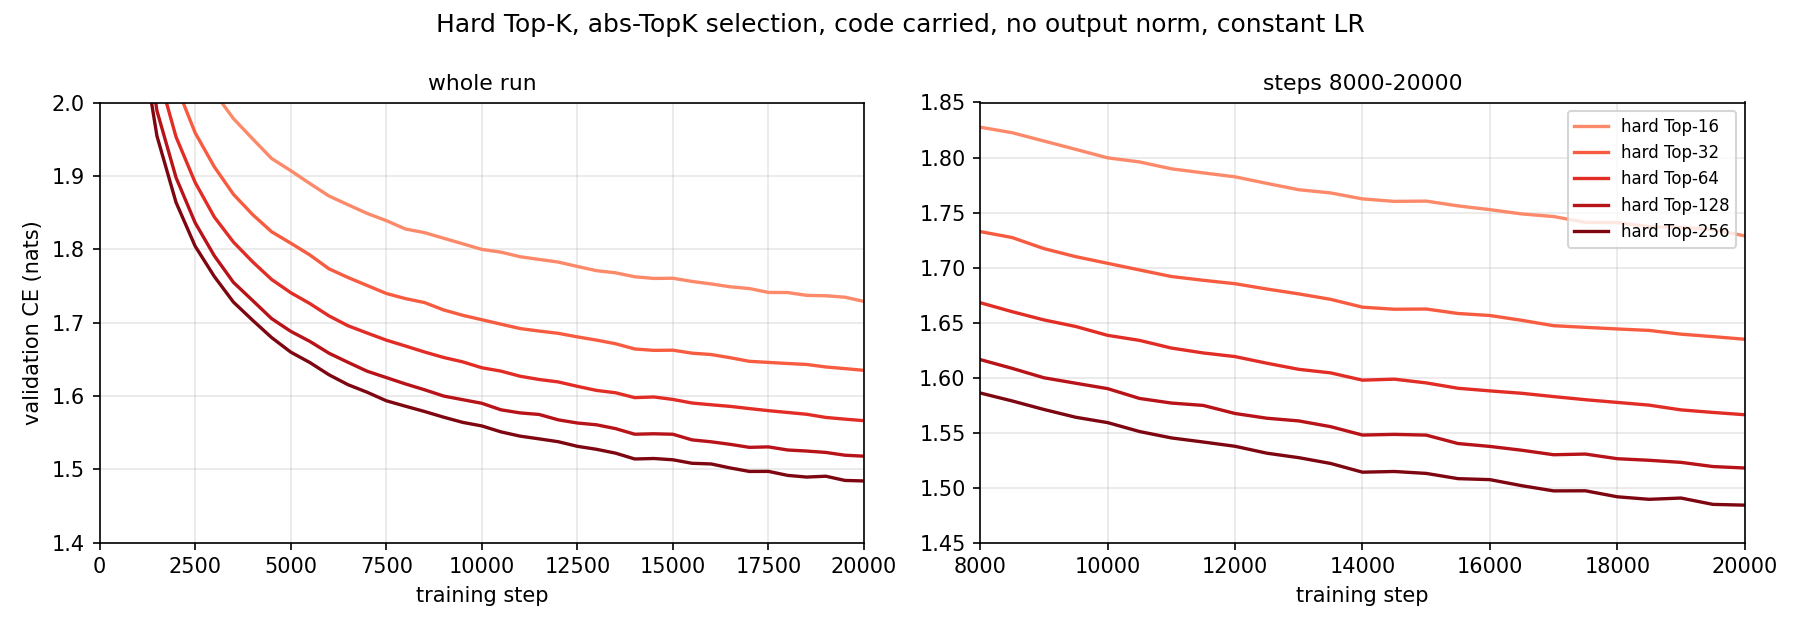
\includegraphics[width=\textwidth]{figures/gumbel-cr/hard_ladder.png}
  \caption{Hard Top-$K$, $K = 16$ to 256: the whole run, and steps 8000--20000.}
  \label{fig:hard}
\end{figure}

Final validation CE: $1.7288$, $1.6348$, $1.5662$, $1.5178$, $1.4840$ for
$K = 16, 32, 64, 128, 256$; each doubling of $K$ lowers the loss by $0.094$,
$0.069$, $0.048$ and $0.034$ nats (Figure~\ref{fig:hard}).

% ============================================================
\section{The $(\tau, \lambda)$ search}
% ============================================================

\begin{figure}[h]
  \centering
  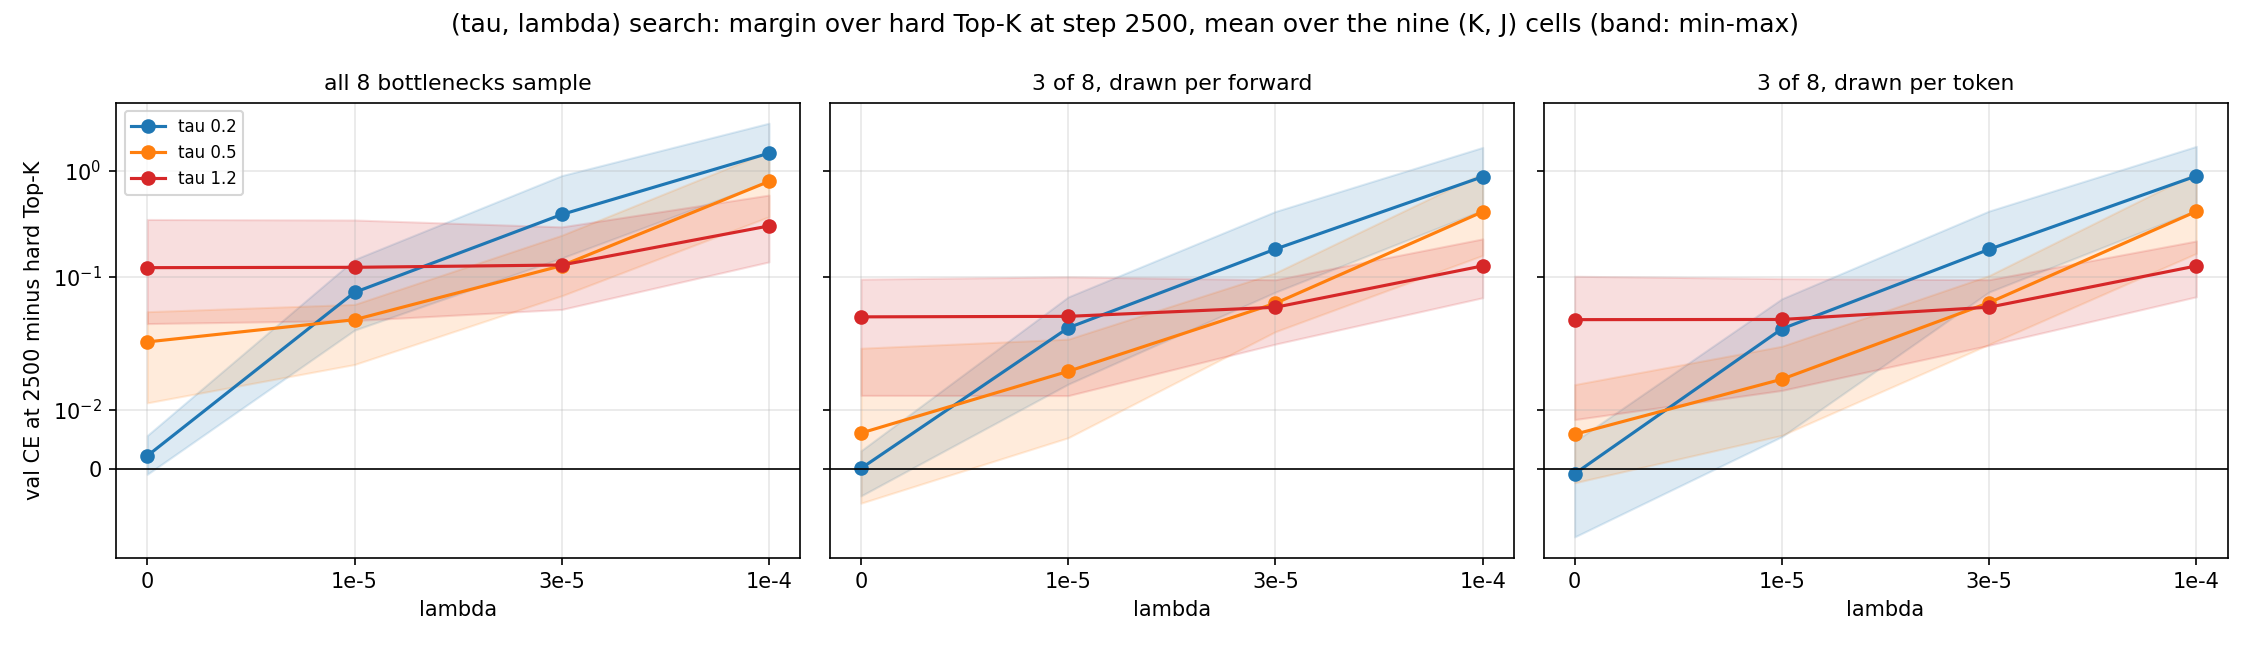
\includegraphics[width=\textwidth]{figures/gumbel-cr/search.png}
  \caption{Validation CE at step 2500 minus hard Top-$K$ at step 2500, mean over
  the 9 cells (band: minimum to maximum over cells), symmetric-log scale.}
  \label{fig:search}
\end{figure}

\textbf{$\lambda$.} The loss rises with $\lambda$ at every $\tau$
(Figure~\ref{fig:search}). The norm of the policy term's gradient, relative to the
CE gradient on the same micro-batch, scales with $\lambda$: median $0.09$, $0.28$
and $0.9$--$1.6$ at $\lambda = 10^{-5}, 3\cdot10^{-5}, 10^{-4}$ with all 8
bottlenecks sampling, about $0.6$ times that with 3 of 8. At $\lambda = 10^{-2}$
it reached $10^{2}$--$10^{3}$: with the gradient clipped at norm 1, the CE
gradient then all but vanishes from the update, the code's scale grows until
sampling is deterministic, and the loss returns to the unigram level.

\textbf{$\tau$.} At $\lambda = 0$ the noise alone costs nothing at $\tau = 0.2$
(mean margin $+0.002$, $0.000$ and $-0.001$ for the three variants), little at
$\tau = 0.5$ ($+0.024$ with all 8, $+0.006$ with 3 of 8), and $0.04$--$0.12$ at
$\tau = 1.2$. A larger $\tau$ makes the loss less sensitive to $\lambda$ but
adds this cost.

% ============================================================
\section{Final results}
% ============================================================

Validation CE after 20000 steps; columns are the candidate pool $K{+}J$, the
last column hard Top-$K$ at the same $K$, the last row hard Top-$(K{+}J)$.
Selected $(\tau, \lambda)$: $\lambda = 0$ everywhere, $\tau = 0.2$ except
$\tau = 0.5$ at $(16,16)$ and $(32,32)$ for 3 of 8 per forward and at $(32,32)$
and $(64,64)$ for 3 of 8 per token.

\begin{center}
\small
\begin{tabular}{llccccc}
\toprule
variant & $K$ & $K{+}J = 32$ & $64$ & $128$ & $256$ & hard Top-$K$ \\
\midrule
all 8 sample        & 16 & 1.7381 & 1.7403 & 1.7432 & 1.7436 & 1.7288 \\
                    & 32 & --     & 1.6394 & 1.6493 & 1.6476 & 1.6348 \\
                    & 64 & --     & --     & 1.5741 & 1.5840 & 1.5662 \\
\midrule
3 of 8, per forward & 16 & 1.7387 & 1.7351 & 1.7368 & 1.7335 & 1.7288 \\
                    & 32 & --     & 1.6418 & 1.6376 & 1.6390 & 1.6348 \\
                    & 64 & --     & --     & 1.5709 & 1.5733 & 1.5662 \\
\midrule
3 of 8, per token   & 16 & 1.7302 & 1.7316 & 1.7408 & 1.7303 & 1.7288 \\
                    & 32 & --     & 1.6402 & 1.6402 & 1.6337 & 1.6348 \\
                    & 64 & --     & --     & 1.5702 & 1.5728 & 1.5662 \\
\midrule
hard Top-$(K{+}J)$  &    & 1.6348 & 1.5662 & 1.5178 & 1.4840 & \\
\bottomrule
\end{tabular}
\end{center}

No cell is below the hard Top-$K$ of its row by more than $0.0011$
(3 of 8 per token, $(32, 224)$), and no cell is closer than $0.05$ to the hard
Top-$(K{+}J)$ of its column. Differences of $0.01$ between cells are within
what one seed resolves.

\begin{figure}[p]
  \centering
  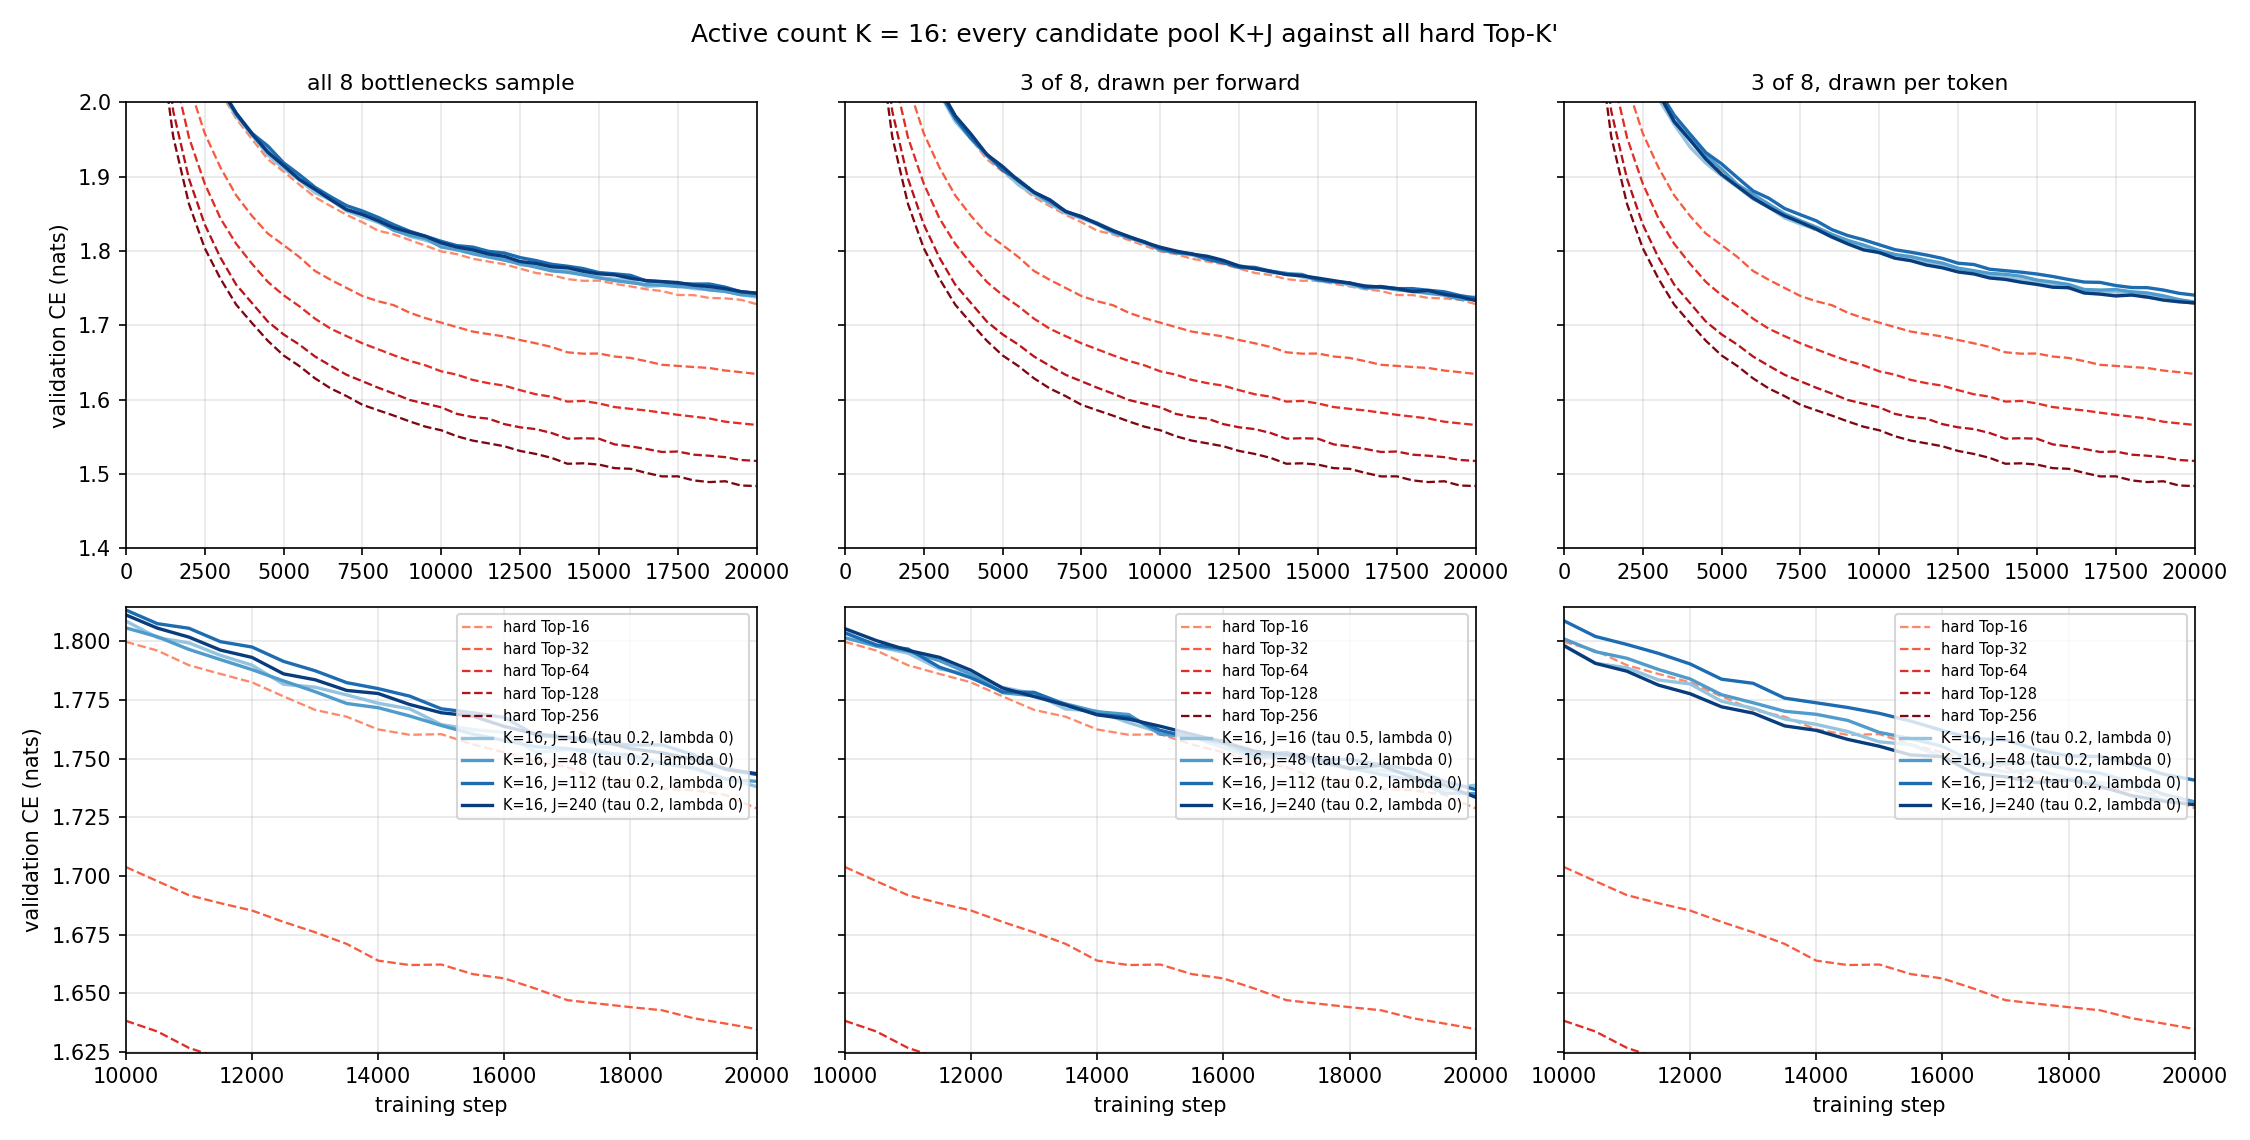
\includegraphics[width=\textwidth]{figures/gumbel-cr/active_k16.png}\\[4pt]
  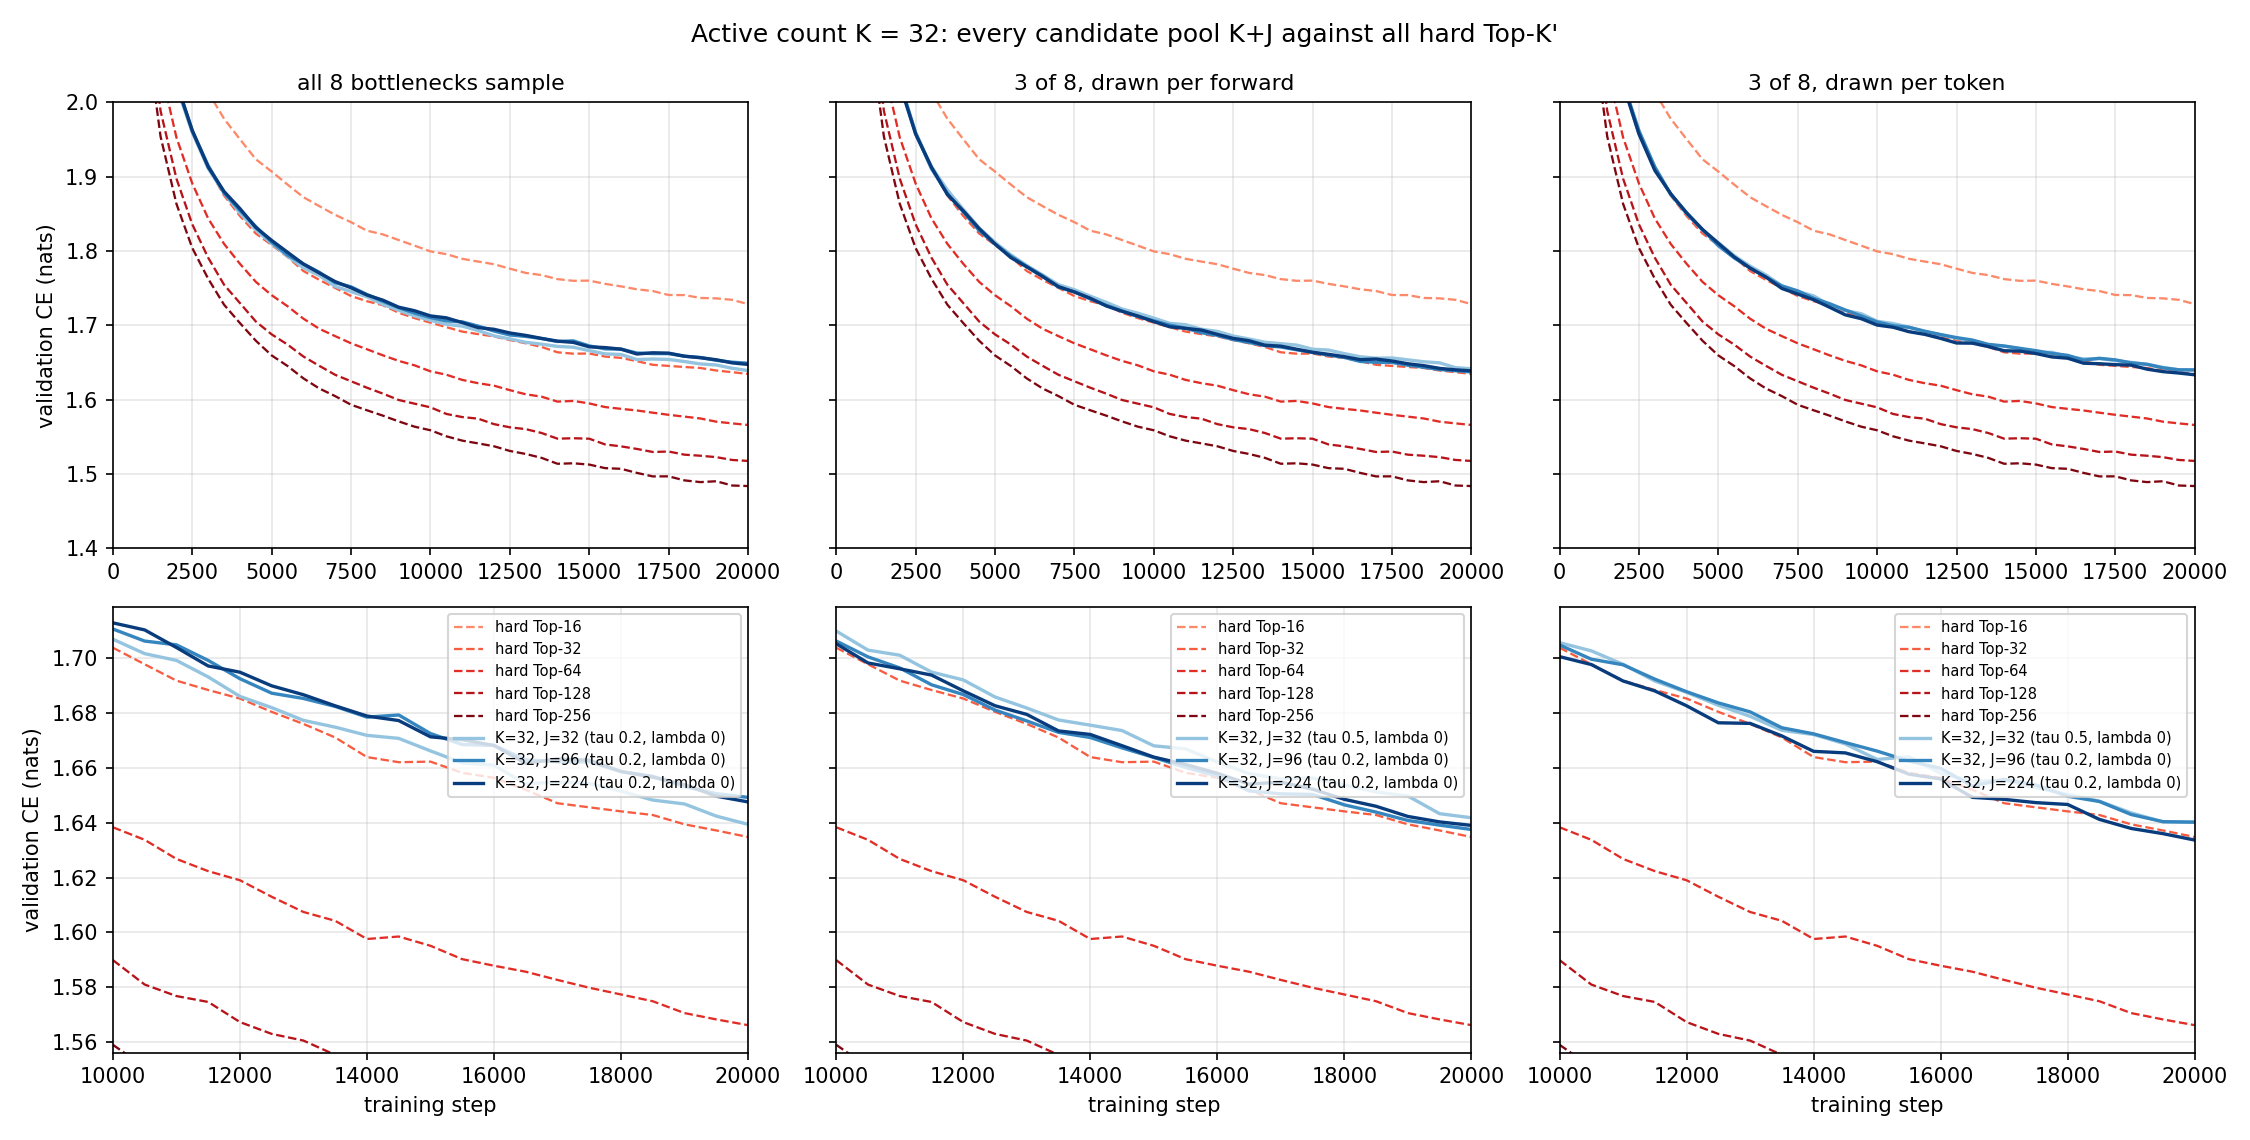
\includegraphics[width=\textwidth]{figures/gumbel-cr/active_k32.png}
  \caption{Per active count, $K = 16$ (top) and $K = 32$ (bottom): every
  candidate pool (solid, blues light to dark with $J$) against all hard
  Top-$K'$ (dashed, reds light to dark with $K'$); one column per variant;
  top rows the whole run, bottom rows steps 10000--20000 between hard Top-$2K$
  and hard Top-$K$. Every Gumbel curve runs along hard Top-$K$.}
  \label{fig:k16k32}
\end{figure}

\begin{figure}[p]
  \centering
  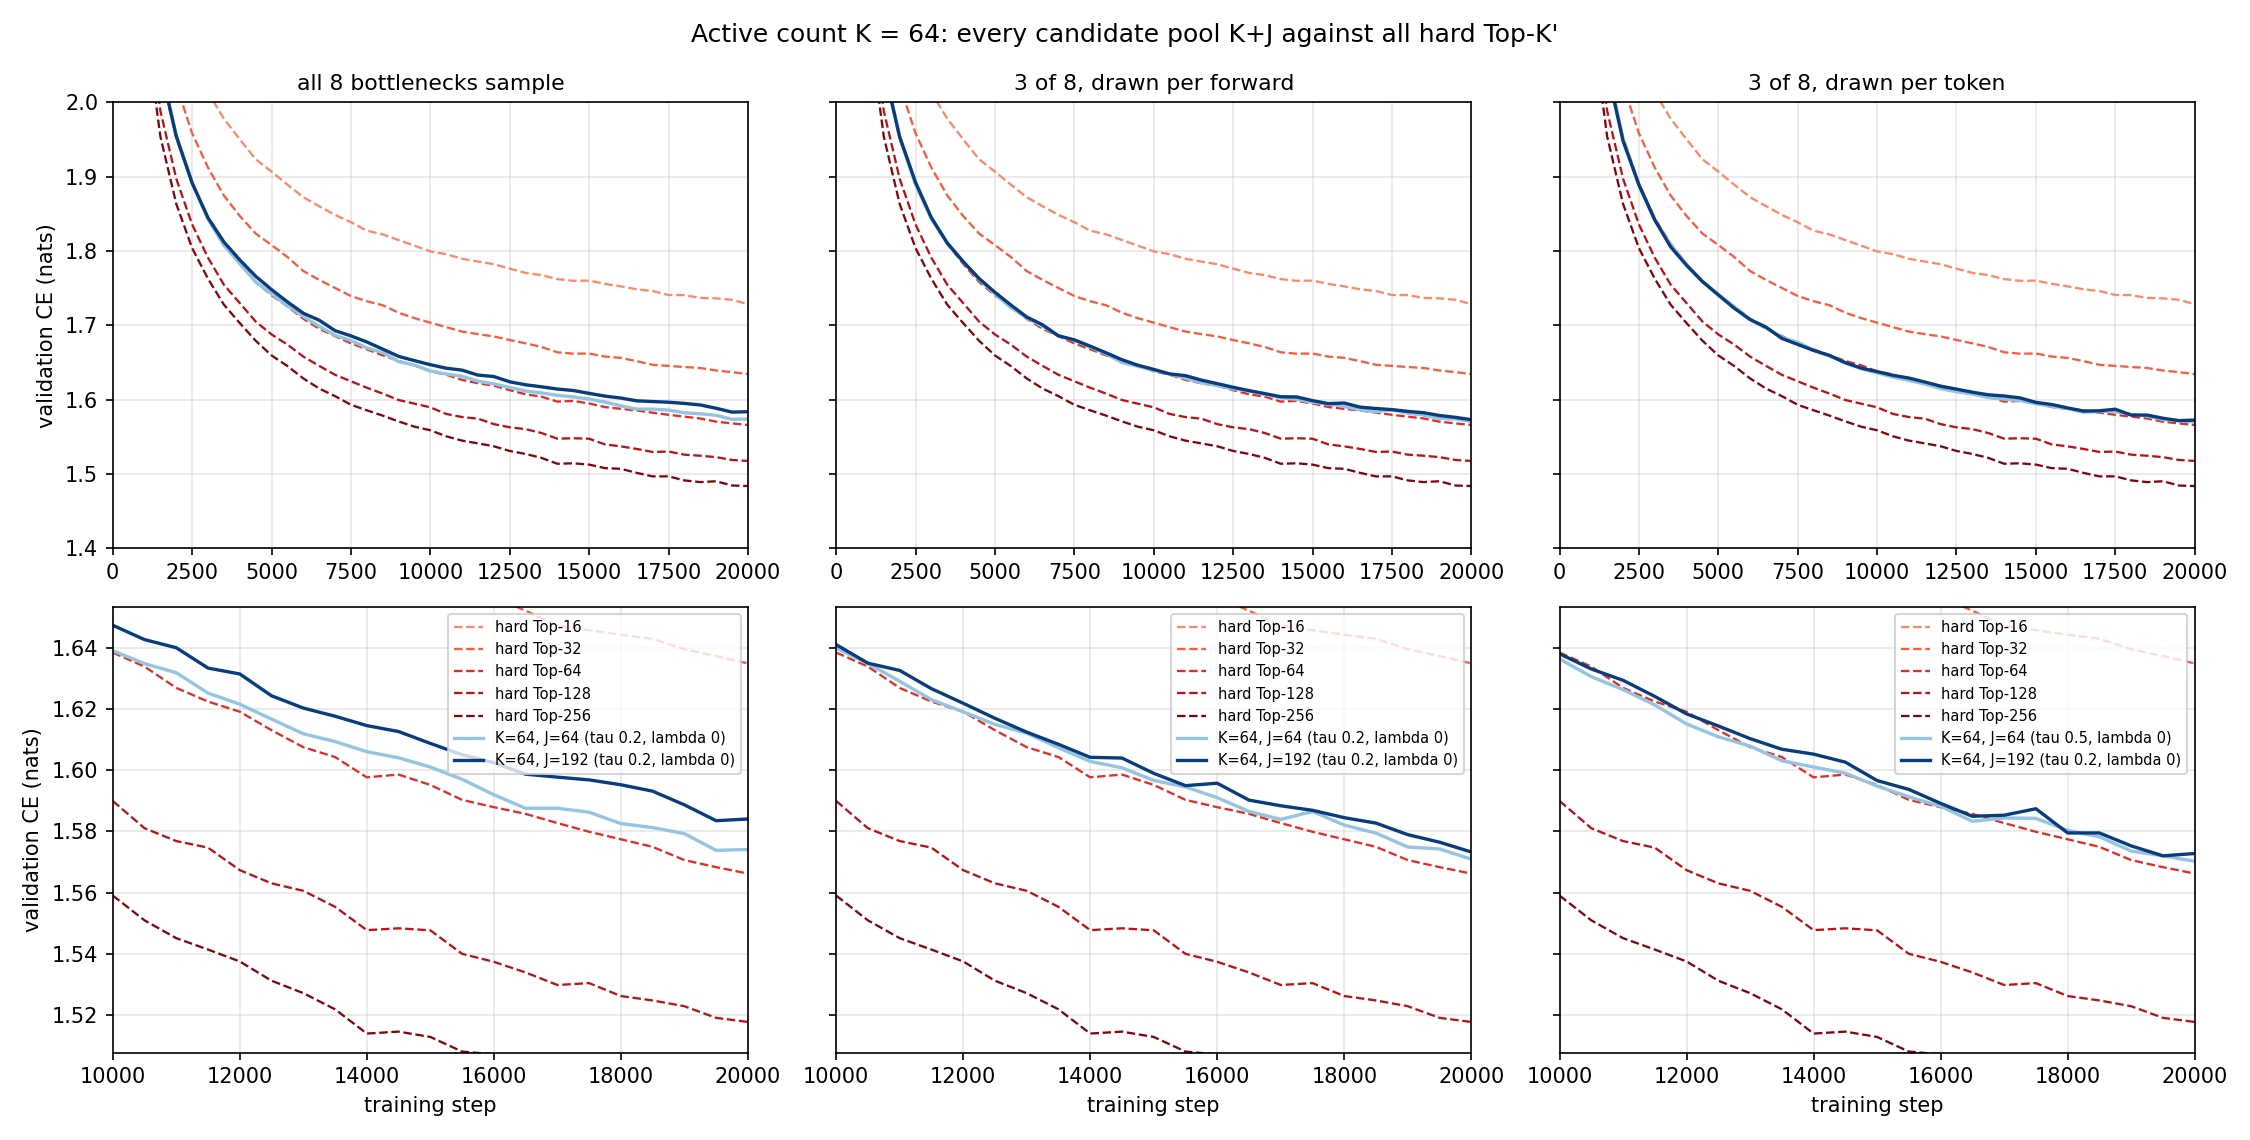
\includegraphics[width=\textwidth]{figures/gumbel-cr/active_k64.png}\\[4pt]
  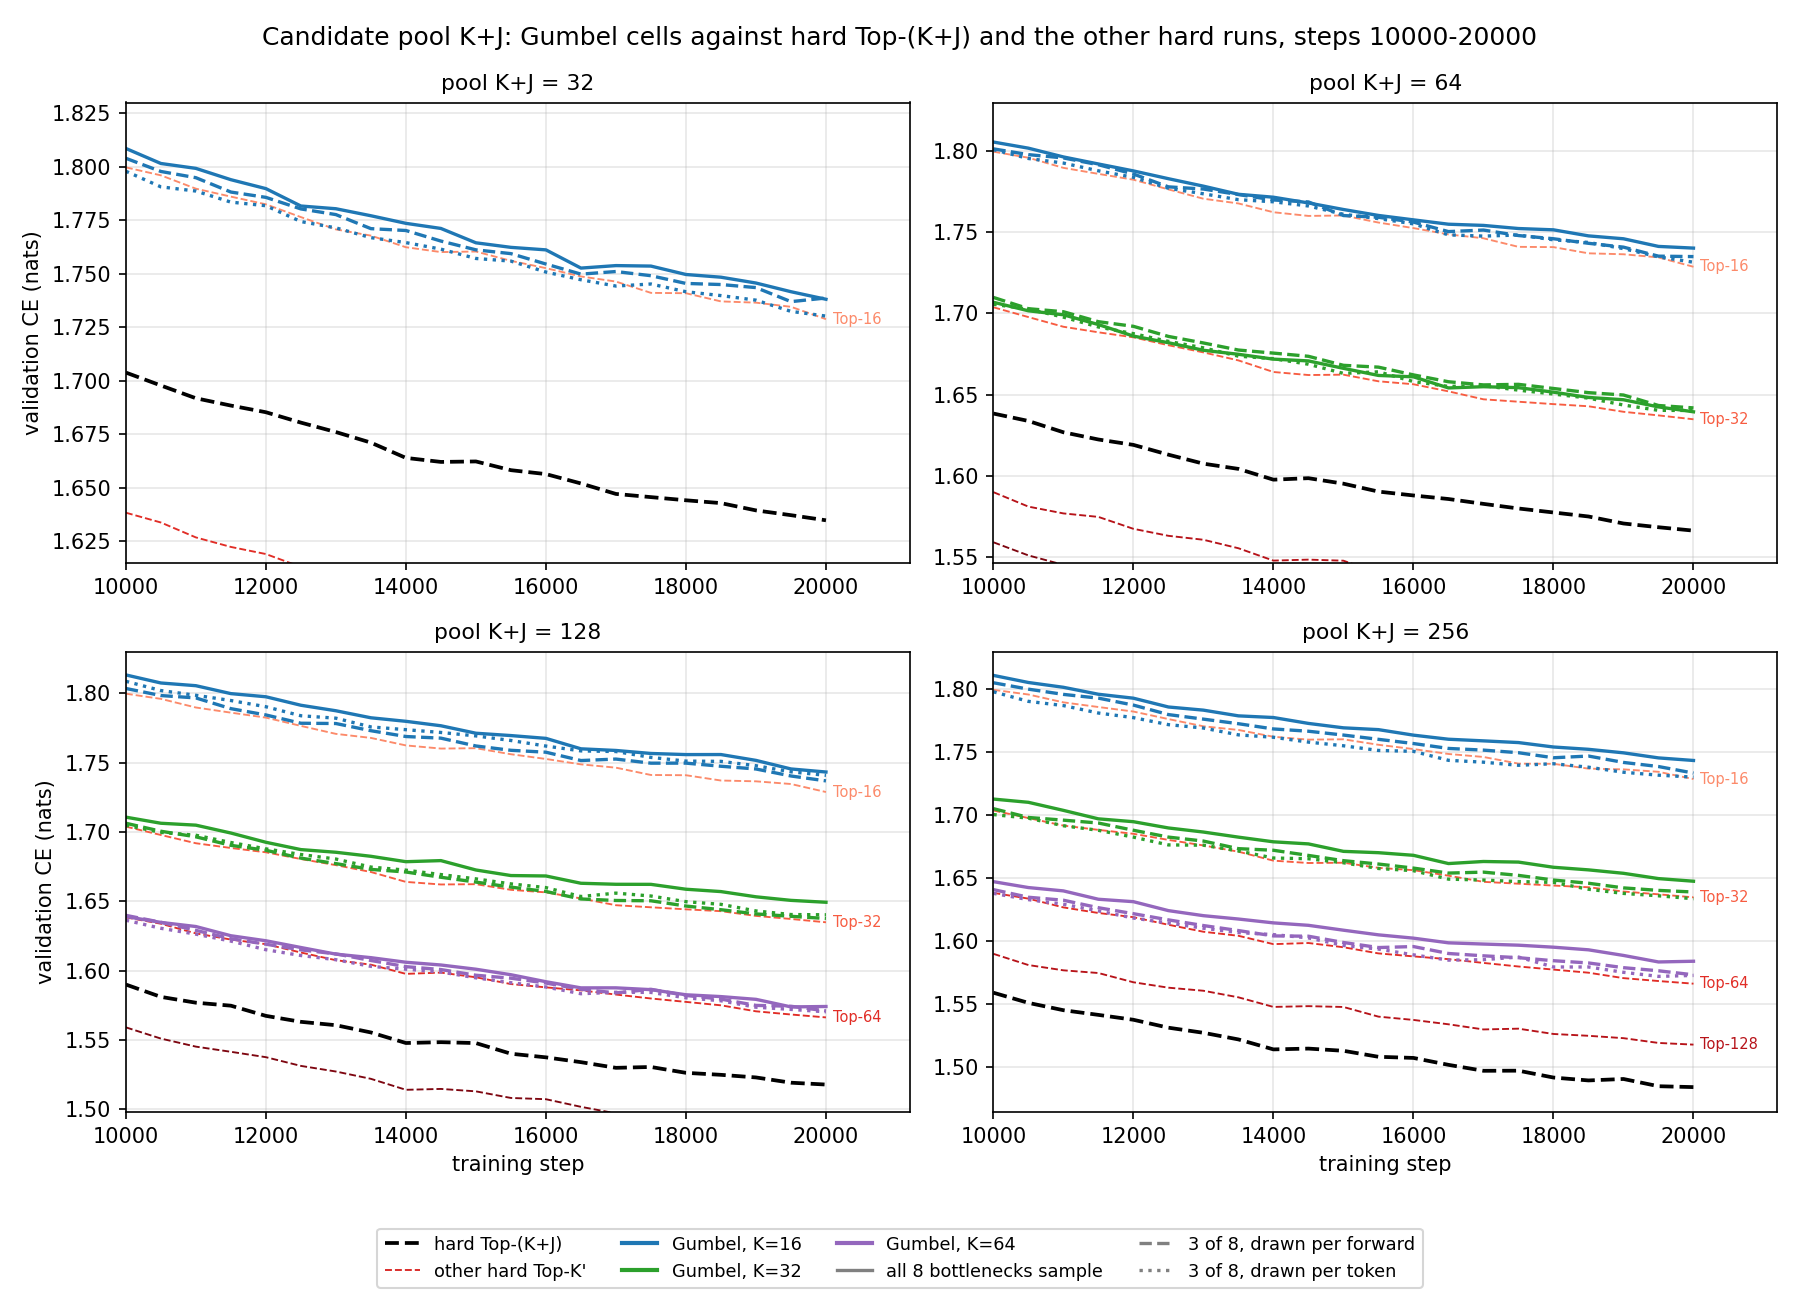
\includegraphics[width=.92\textwidth]{figures/gumbel-cr/pools.png}
  \caption{Top: $K = 64$, as in Figure~\ref{fig:k16k32}. Bottom: per candidate
  pool $K{+}J$, the Gumbel cells with that pool (color: $K$; line style:
  variant) against hard Top-$(K{+}J)$ (black dashed) and the other hard runs.
  Each Gumbel cell lies on the hard curve of its own $K$, not near that of its
  pool.}
  \label{fig:k64pools}
\end{figure}

% ============================================================
\section{The noise does not die out}
% ============================================================

\begin{figure}[h]
  \centering
  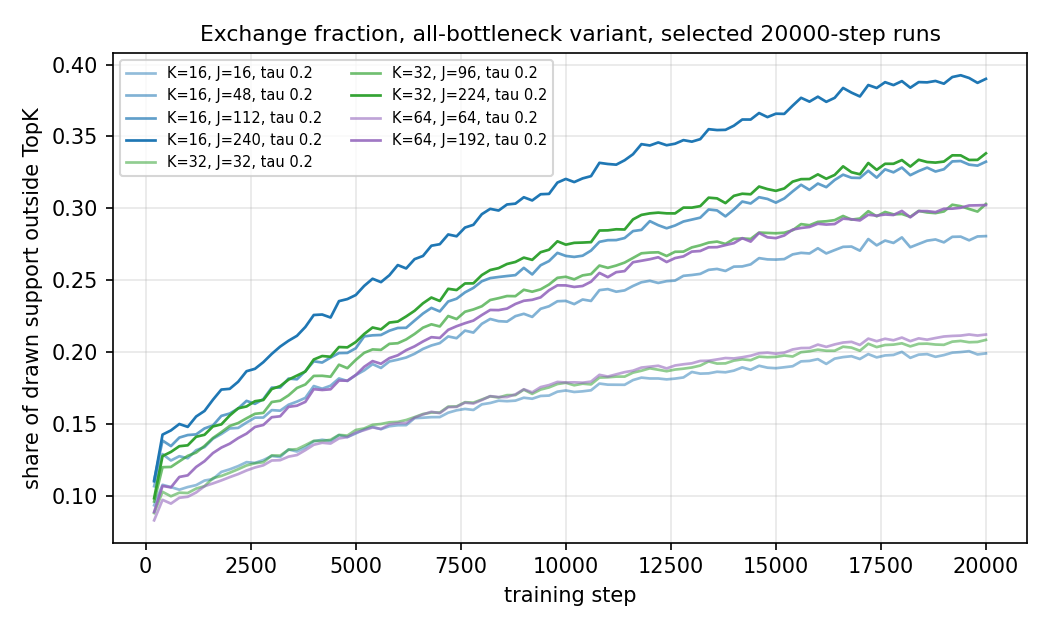
\includegraphics[width=.62\textwidth]{figures/gumbel-cr/exchange.png}
  \caption{Share of the drawn support outside the deterministic Top-$K$ during
  the selected 20000-step runs, all 8 bottlenecks sampling, $\tau = 0.2$,
  $\lambda = 0$.}
  \label{fig:exchange}
\end{figure}

In the selected runs the share of the drawn support outside the deterministic
Top-$K$ grows during training, from $0.08$--$0.11$ at step 200 to $0.20$--$0.39$
at step 20000, more for larger $J$ (Figure~\ref{fig:exchange}). The model does
not escape the noise by enlarging the gaps between scores; the loss is
nevertheless that of hard Top-$K$.

% ============================================================
\section{Interpretation}
% ============================================================

The simplest reading: with $\lambda = 0$ a Gumbel Top-$(K{+}J)$ bottleneck is
hard Top-$K$ with random exchanges near the $K$-th score. Exchanges between
coordinates of similar magnitude cost nothing measurable, and the forward never
uses more than $K$ coordinates, so the model cannot gain what hard Top-$(K{+}J)$
gains. The policy gradient is the only term that reaches the candidates outside
the drawn support, but its estimate is dominated by noise: its norm equals
the CE gradient's near $\lambda = 10^{-4}$, where it already costs $0.3$--$1.5$
nats at step 2500 (mean over cells, depending on $\tau$), and at
$\lambda = 10^{-5}$, a tenth of the CE gradient, it still costs
$0.015$--$0.07$ nats and improves no cell. Sampling at 3
of 8 bottlenecks lowers that noise by about the factor the gradient ratios show,
not enough to change the outcome.

% ============================================================
\section{Scope}
% ============================================================

Single runs at seed 1337, on two boxes of the same GPU type; differences of
$0.01$ nats are within run-to-run variation. Constant learning rate, so the
absolute values are not comparable with the cosine-schedule K+J notes. abs-TopK
selection only. The $(\tau, \lambda)$ search ranks settings at step 2500; the
settings that lost there were not continued, so an advantage appearing only
later in training is not excluded.

{\raggedright\textbf{Data.} Runs on Drive \code{runs\_ankara} (all 8; 3 of 8 per forward;
hard Top-$K$) and \code{runs\_bern} (3 of 8 per token; the remaining
all-8 cells); selections in \code{analysis\_\{ankara,bern\}/gcr\_selection\_*.json}
and \code{docs/figures/gumbel-cr/data/}; figures and tables:
\code{scripts/plot\_gumbel\_cr\_report.py}.\par}

\end{document}
